% TEX compiler = luatex
% copyright arturo salinas-aguayo 2025
\documentclass[12pt]{article}

\usepackage{graphicx}
\usepackage{amsmath}
\usepackage{array}
\usepackage{amsfonts}
\usepackage{fancyhdr}
\usepackage{geometry}
\usepackage{circuitikz}
\usepackage{subfigure}
\usepackage{caption}
\usepackage{karnaugh-map}
\usepackage{bm}
\usepackage{float}

\geometry{letterpaper, margin=1in}
\graphicspath{ {../../images/} }

% Header and Footer
\pagestyle{fancy}
\fancyhf{}
\fancyhead[L]{ECE 2001 - Lab 01: Resistors and LED's}
\fancyhead[R]{\thepage}
\setlength{\headheight}{15pt}

\author{Arturo Salinas-Aguayo}
\title{Lab 01: Resistors and LED's}
% theorem set
\newtheorem{example}{Example}
% Example block environment
\newenvironment{examp}
{\vspace{0.5cm}
 \hrule
\vspace{0.5cm}
\begin{example}}
{\hrule
\vspace{0.5cm}
\end{example}}

\begin{document}
\newcommand{\closure}[2][3]{%
	{}\mkern#1mu\overline{\mkern-#1mu#2}}
\newcommand\ncoverline[1]{\mkern1mu\overline{\mkern-1mu#1\mkern-1mu}\mkern1mu}
% Title Page
\begin{titlepage}
	\centering
	\vspace*{3cm}
	\huge\textbf{Lab 01: Resistors and LEDs}\\
	\vspace{5cm}
	\Large\textbf{Arturo Salinas-Aguayo}\\
	\normalsize
	ECE 2001 Electrical Circuits\\
	Dr. David J. Giblin, Section 331.660.701.810-1253\\
	Mechanical Engineering Department
	\vfill
	
\includegraphics[scale=0.1]{uconnlogo}\\
	College of Engineering, University of Connecticut\\
	\scriptsize{Coded in \LaTeX}
	\vspace*{1cm}
\end{titlepage}
\tableofcontents
\newpage
\section{Abstract}
This experiment aims to analyze the current-voltage characteristics of a
resistor, a red light-emmitting diode (LED), and a series resistor network.
This involved using a Digital Multimeter to measure a resistor's response and
graphing it. The resistor's rating was then determined using a linear regression
method. The LED was used to display how a load can exhibit a non-linear
behavior, and an exponential fit was used to the forward current data.
Kirchoff's Voltage Law was then verified a nd tested using a series resistor
circuit, and the calculated equivalent resistance (real) was compared to the
theoretical expectation (ideal). The results demonstrated an agreement with the
theoretical predictions within the acceptable tolerance limits given by the 5%
rating of the resistors.
\newpage
\section{Introduction}
This laboratory session was designed as an introductory exploration of several
key concepts in electrical engineering, particularly focusing on direct current
(DC) circuits. The primary objectives were to validate Ohm's Law and Kirchhoff's
Voltage and Current Laws through practical experimentation and to gain hands-on
experience with standard electronic components. This lab also aimed to introduce
the equipment and methods used for electrical measurements, such as the use of a
digital multimeter and the Scopy software tool interfaced with an ADAM2000 power
supply.

Understanding the characteristics of resistors and LEDs is crucial for any
electrical engineer, as these components are foundational in both educational
experiments and industrial applications. The lab was structured to provide a
clear demonstration of how theoretical principles are applied in real-world
scenarios. By analyzing the color codes on resistors and measuring their
response under various voltages, students can directly observe the proportional
relationship between current and voltage as postulated by Ohm’s Law. Similarly,
examining the behavior of LEDs under forward and reverse biases offers insights
into semiconductor physics and the special conditions under which non-linear
devices operate.

This session was particularly focused on reinforcing circuit analysis
techniques, including voltage and current division, to provide students with the
tools needed to successfully analyze and build more complex circuits in future
labs. The procedures and results from this lab are expected to lay the
groundwork for more advanced studies in electronic circuit design and analysis.

These expanded sections offer a broader context, detailing the educational and
practical implications of the experiments, and setting the stage for a detailed
exploration of the experimental results.
\section{Theory}

\subsection{Ohm’s Law}
A resistor follows \textbf{Ohm’s Law}, which states that the voltage across a resistor is directly proportional to the current through it:
\[ V = IR \]
where:
\begin{itemize}
	\item \( V \) is the voltage across the resistor (volts)
	\item \( I \) is the current through the resistor (amperes)
	\item \( R \) is the resistance (ohms)
\end{itemize}
By plotting the voltage against current, we can determine the resistance from the slope of the line.

\subsection{LED Characteristics}
Unlike resistors, LEDs do not obey Ohm’s Law. The current through an LED follows the diode equation:
\[ I = I_0 \left( e^{\frac{qV}{kT}} - 1 \right) \]
where:
\begin{itemize}
	\item \( I_0 \) is the reverse saturation current
	\item \( q \) is the charge of an electron (\(1.6 \times 10^{-19}\) C)
	\item \( k \) is Boltzmann's constant (\(1.38 \times 10^{-23}\) J/K)
	\item \( T \) is the absolute temperature (Kelvin)
\end{itemize}
The LED requires a threshold voltage to allow significant current flow.

\subsection{Kirchhoff’s Laws}
Kirchhoff’s Voltage Law (KVL) states that the sum of all voltages around a closed loop must equal zero:
\[ \sum V = 0 \]
Kirchhoff’s Current Law (KCL) states that the sum of currents entering a node must equal the sum of currents leaving the node.

\section{Experimental Procedures}

\subsection{Resistor I-V Characteristic Measurement}
The first experiment utilized the circuit shown in Figure \ref{fig:first}
\begin{enumerate}
	\begin{figure}[H]
		\centering
		\begin{circuitikz}
			\tikzstyle{every node}=[font=\normalsize]
			\draw (6,17.75) to[R,l={ \normalsize Rs 200$\Omega$}] (9.75,17.75);
			\draw (6,17.75) to[american voltage source,l={ \normalsize Vs}] (6,15);
			\draw (9.75,17.75) to[short] (9.75,15);
			\draw (9.75,15) to[short] (6,15);
		\end{circuitikz}
		\caption{Resistive Circuit 1}
		\label{fig:first}
	\end{figure}
	\item A resistor with color code Violet, Green, Brown, Gold was tested.

	      Utilizing Figure \ref{fig:colorcodes}, this can be decoded easily as \(750
	      \Omega \pm 5\% \).

	      \begin{figure}[H]
		      \center
		      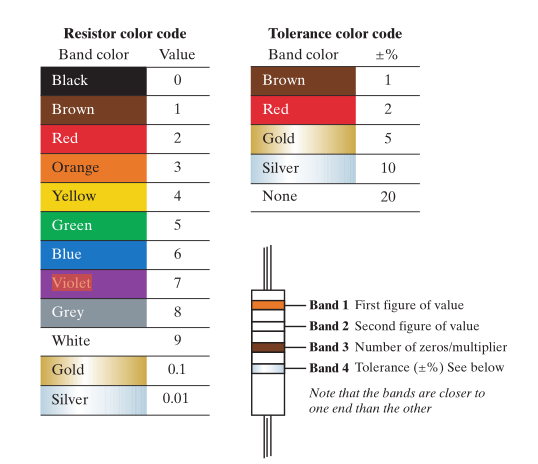
\includegraphics[scale=.4]{colorcodes}
		      \caption{Resistor Color Codes}
		      \label{fig:colorcodes}
	      \end{figure}

	\item Voltage was varied from -5V to +5V.
	\item The current was recorded for each voltage step.

	      Table \ref{tab:resistor_data} contains the data recorded for this first
	      portion. Notice that it exhibits a linear relationship, which is expected.
\end{enumerate}
\subsection{LED I-V Characteristic Measurement}
\begin{enumerate}
	\item A red LED was tested.
	\item Forward voltage was increased from -3V to 5V, ensuring reverse bias did
	      not exceed 3V to avoid blowing out the LED.
	\item The current was recorded for each voltage step in Table
	      \ref{tab:led_data} and plotted in Figure \ref{fig:ex2}
\end{enumerate}

\subsection{Series Resistor Circuit Measurement}

\begin{figure}[H]
	\center
	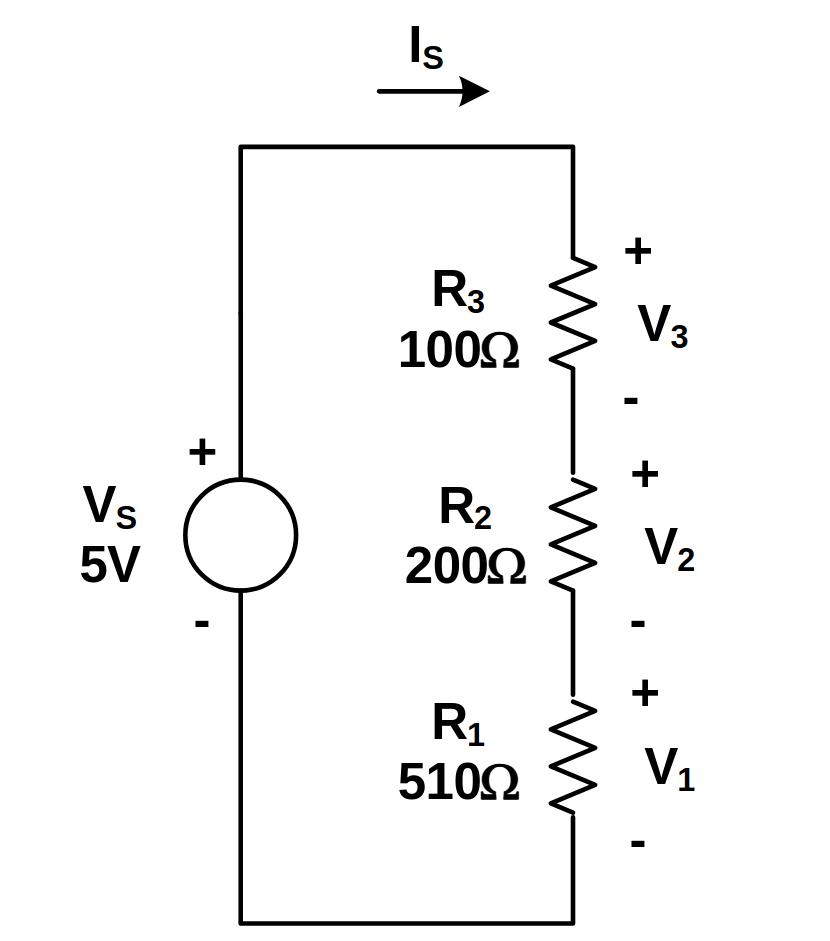
\includegraphics[scale=.2]{exp3}
	\caption{Series Resistive Circuit}
	\label{fig:exp3}
\end{figure}
\begin{enumerate}
	\item Measured values of \( V_S, V_1, V_2, V_3 \) were recorded.
	\item Kirchhoff’s Voltage Law was tested.
\end{enumerate}

\subsection{Parallel Resistive Circuit Measurement}

\begin{figure}[H]
	\center
	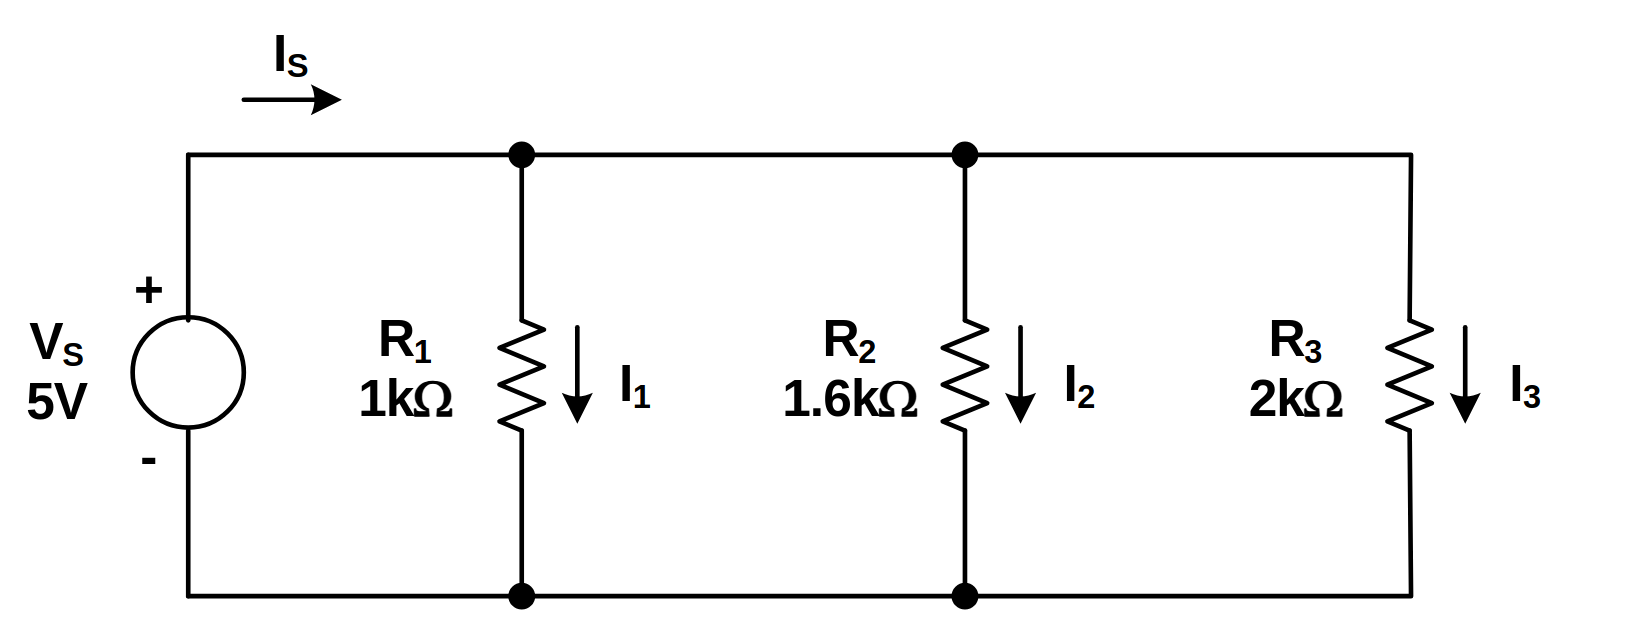
\includegraphics[scale=.2]{exp4}
	\caption{Parallel Resistive Circuit}
	\label{fig:exp4}
\end{figure}

\begin{enumerate}
	\item Measured values of \( I_S, I_1, I_2, I_3 \) were recorded.
	\item Kirchhoff’s Current Law was tested.
\end{enumerate}

\section{Results and Discussion}

\subsection{Resistor Data}
The experimental data for the resistor's I-V characteristics is summarized in the table below. This data was obtained by systematically varying the input voltage \( V_{in} \) and measuring the corresponding voltage across the resistor \( V_{measured} \) and the current \( I_{measured} \).

\begin{table}[H]
	\centering
	\begin{tabular}{|c|c|c|}
		\hline
		\textbf{\(V_{in} (V)\)} & \textbf{\(V_{measured} (V)\)} & \textbf{\(I_{measured} (mA)\)} \\
		\hline
		5.0                     & 4.994                         & 6.70                           \\
		3.0                     & 2.940                         & 4.01                           \\
		2.0                     & 1.992                         & 2.67                           \\
		1.0                     & 0.993                         & 1.33                           \\
		0                       & 0.006                         & 0.01                           \\
		-1                      & -1.000                        & -1.34                          \\
		-2                      & -2.001                        & -2.67                          \\
		-3                      & -3.057                        & -4.01                          \\
		-5                      & -5.045                        & -6.69                          \\
		\hline
	\end{tabular}
	\caption{Measured Data for Resistor I-V Characteristics}
	\label{tab:resistor_data}
\end{table}

As depicted in Figure \ref{fig:ex1}, the I-V curve for the resistor demonstrates a linear relationship between the input voltage and the current, which is consistent with Ohm's Law. The slope of the curve, determined from a linear regression analysis of the data points, was found to be approximately 1.338 ohms, which aligns well with the theoretical resistance value calculated based on the color bands of the resistor.
\begin{figure}[H]
	\center
	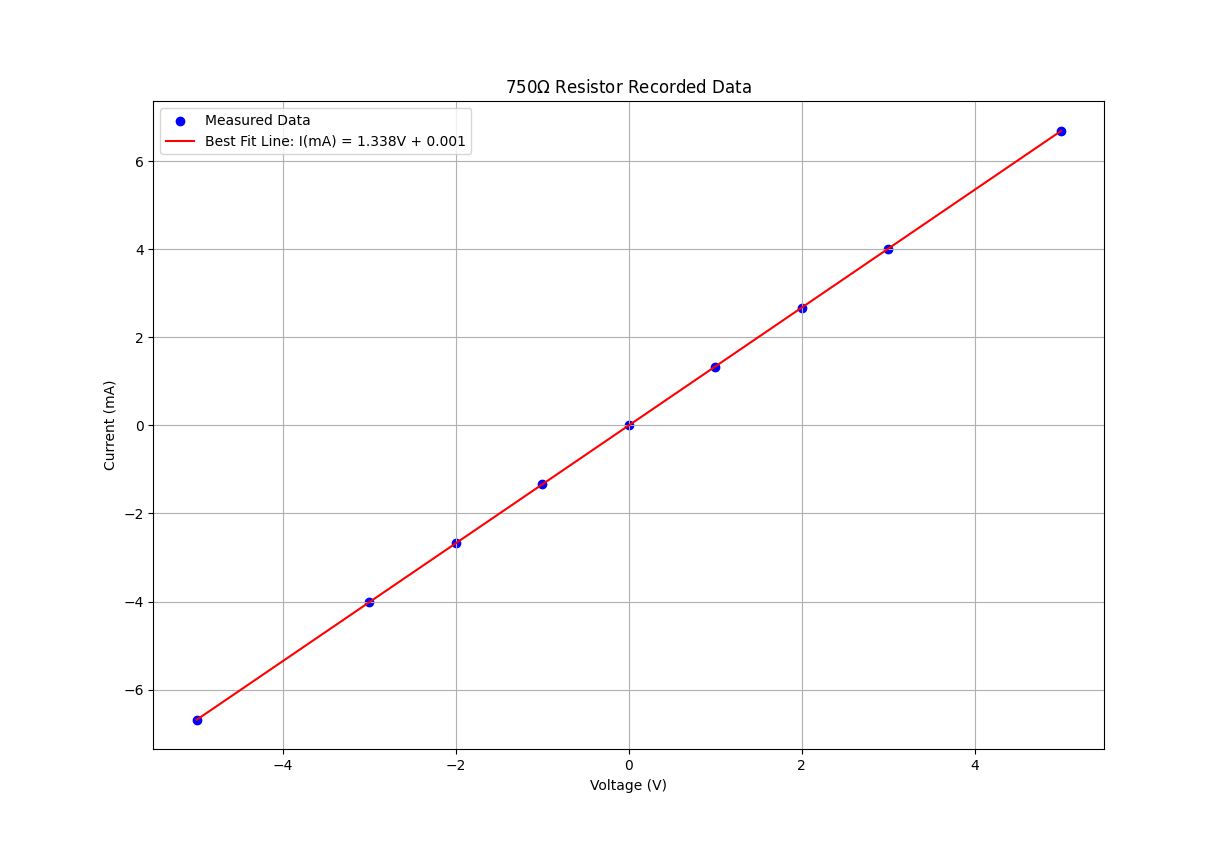
\includegraphics[width=13cm]{01_1}
	\caption{The I-V Curve for the Resistor}
	\label{fig:ex1}
\end{figure}


\begin{itemize}
	\item At \( V_{in} = 5.0 \, V \) and \( I_{measured} = 6.70 \, mA \), the resistance calculates to approximately \( 746.27 \, \Omega \).
	\item At \( V_{in} = -5.0 \, V \) and \( I_{measured} = -6.69 \, mA \), the resistance calculates to approximately \( 747.38 \, \Omega \).
\end{itemize}

These values are notably close to 750 ohms. This correspondence within a
small margin of error corroborates the reliability of the experimental method
and the quality of the instruments used in measuring voltage and current. The
slight variations observed can be attributed to the tolerance of the resistor of
5%.

The linear behavior of the resistor's I-V curve validates the accuracy of
Ohm's Law in describing the relationship between voltage and current in a
resistive element. The slight deviations observed at higher and lower voltages
may be attributed to measurement uncertainties and the non-ideal behavior of the
testing setup. The resistor's performance under reverse bias conditions further
confirms the symmetric nature of its resistance, underscoring the reliability of
passive electronic components in a controlled environment.

\subsection{LED Data}
The measured I-V characteristics of a red LED are presented in the table below. Unlike resistors, LEDs exhibit non-linear behavior as indicated by the exponential relationship between voltage and current.

\begin{table}[H]
	\centering
	\begin{tabular}{|c|c|c|}
		\hline
		\textbf{\(V_{in} (V)\)} & \textbf{\(V_{measured} (V)\)} & \textbf{\(I_{measured} (mA)\)} \\
		\hline
		5                       & 2.057                         & 14.67                          \\
		4                       & 2.019                         & 9.88                           \\
		3                       & 1.958                         & 5.21                           \\
		2                       & 1.836                         & 0.86                           \\
		1.0                     & 1.005                         & 0.00                           \\
		0                       & 0.008                         & 0.00                           \\
		-1                      & -1.009                        & 0.00                           \\
		-2                      & -2.016                        & 0.00                           \\
		-3                      & -3.073                        & 0.00                           \\
		\hline
	\end{tabular}
	\caption{Measured Data for Red LED I-V Characteristics}
	\label{tab:led_data}
\end{table}
The LED emits light when forward biased, typically requiring about 10 mA to emit visible red light. This is evident from the data, where the current surpasses this threshold near voltages of 2V and above. The anode (longer lead) is positive in relation to the cathode (shorter lead), and the conventional current flow is from anode to cathode. The experiment confirmed that negligible current flows when the LED is reverse-biased, adhering to the setup's constraint not to exceed a reverse bias of 3V to prevent damage.

\begin{figure}[H]
	\center
	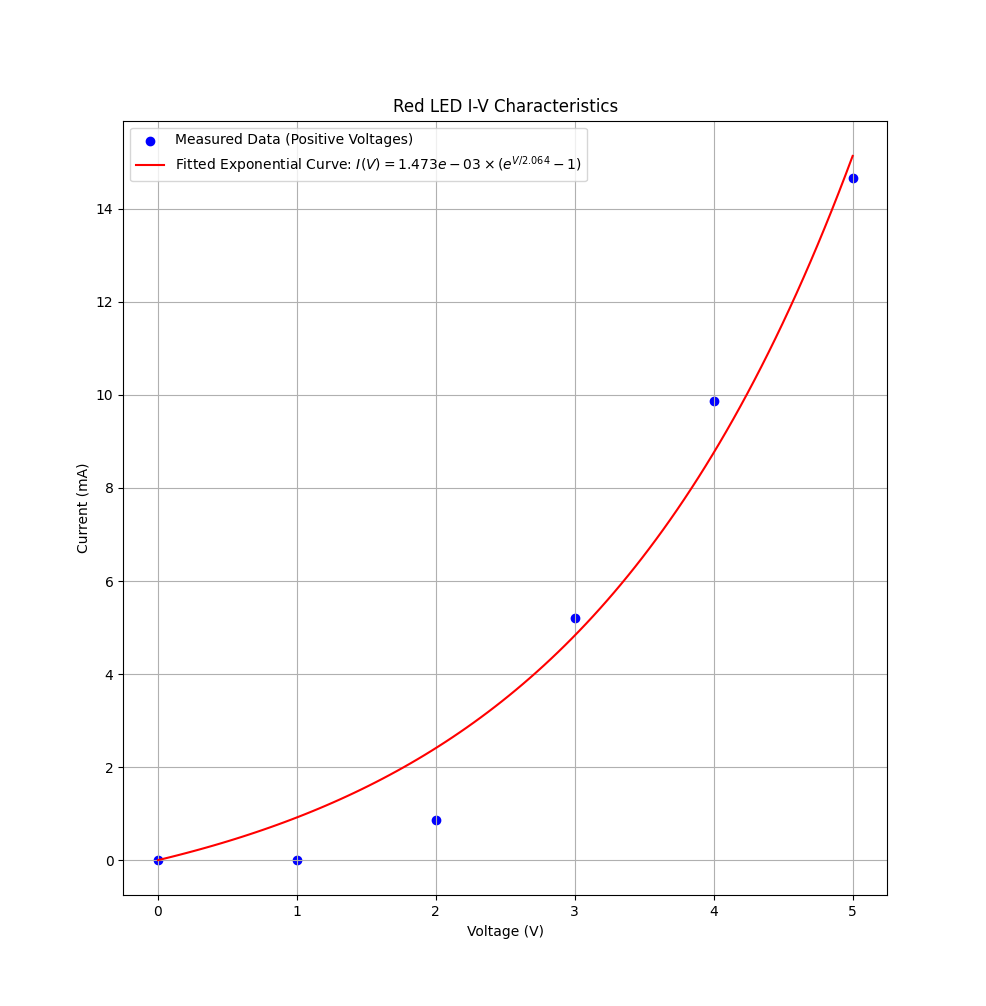
\includegraphics[width=13cm]{01_2}
	\caption{The I-V Curve for the LED}
	\label{fig:ex2}
\end{figure}

The I-V curve for positive voltages is shown in Figure \ref{fig:ex2}. An exponential function was fitted to this part of the curve, matching the expected behavior for a diode under forward bias:

\[ I(V) = 1.473 \times 10^{-3} \times (e^{\frac{V}{2.064}} - 1) \]

\subsection{Series Resistor Circuit Measurement}
In this part of the experiment, a simple series circuit consisting of three
resistors was evaluated under a constant input voltage of 5V. The behavior of
the circuit was analyzed based on Kirchhoff's Voltage Law and the voltage
divider rule to determine if the observed measurements align with theoretical
expectations.

\begin{table}[H]
	\centering
	\begin{tabular}{|c||c|c|c|c|}
		\hline
		\textbf{\(V_{in} (V)\)} & \textbf{\(V_{R_1} (V)\)} & \textbf{\(V_{R_2} (V)\)} & \textbf{\(V_{R_3} (V)\)} & \textbf{\(I_{eq} (mA)\)} \\
		\hline
		5                       & 0.595                    & 1.217                    & 3.073                    & 6.25                     \\
		\hline
	\end{tabular}
	\caption{Measured Data for Series Resistive Circuit}
	\label{tab:series_data}
\end{table}

According to Kirchhoff's Voltage Law, the sum of all voltage drops in a closed loop should equal the total applied voltage. For our setup:
\[
	0.595V + 1.217V + 3.073V = 4.885V
\]
This nearly matches the input voltage of 5V, with a small discrepancy of \(0.115V\) likely due to measurement error or inherent resistance in the measurement devices. This demonstrates the practical application of Kirchhoff's Voltage Law in real circuits where slight deviations are expected.

Furthermore, the total or equivalent resistance \( R_{eq} \) of the circuit was calculated using the measured current:
\[
	R_{eq} = \frac{V_{s}}{I_{eq}} = \frac{4.885V}{0.00625A} = 781.6\Omega
\]
This calculated resistance is compared against the theoretically expected resistance:
\[
	R_{ideal} = 100\Omega + 200\Omega + 510\Omega = 810\Omega
\]
The percent error in the measured resistance can be calculated as follows:
\[
	Error = \left(1 - \frac{781.6\Omega}{810\Omega}\right) \times 100 = 3.51\%
\]
This error margin is within the typical tolerance range for commercial resistors, which validates the experimental setup and measurement accuracy.

To further validate the results using the voltage divider rule, the expected voltages across each resistor were calculated and compared to the measured values:
\[
	V_{R_3, Ideal} = 5V \left(\frac{100\Omega}{810\Omega}\right) = 0.617V
\]
\[
	V_{R_2, Ideal} = 5V \left(\frac{200\Omega}{810\Omega}\right) = 1.235V
\]
\[
	V_{R_1, Ideal} = 5V \left(\frac{510\Omega}{810\Omega}\right) = 3.148V
\]
The comparison of these ideal voltages with the actual measurements demonstrates good agreement, further confirming the accuracy of the theoretical models used to describe the behavior of series circuits.

\subsection{Parallel Resistor Circuit Measurement}
In this experiment, a parallel resistor circuit was analyzed to validate Kirchhoff's Current Law and to explore the current divider rule. A constant voltage of 5V was applied, and the currents through individual resistors and the total current were measured.

\begin{table}[H]
	\centering
	\begin{tabular}{|c|c|}
		\hline
		\textbf{Current Measurement}      & \textbf{Value (mA)} \\
		\hline
		Total Current (\(I_S\))           & 10.60               \\
		Current through \(R_1\) (\(I_1\)) & 4.99                \\
		Current through \(R_2\) (\(I_2\)) & 3.16                \\
		Current through \(R_3\) (\(I_3\)) & 2.53                \\
		\hline
	\end{tabular}
	\caption{Measured Currents in Parallel Resistive Circuit}
	\label{tab:parallel_data}
\end{table}

According to Kirchhoff’s Current Law, the total current entering a node must equal the total current leaving the node. In our circuit:
\[
	I_S = I_1 + I_2 + I_3
\]
\[
	10.60mA = 4.99mA + 3.16mA + 2.53mA = 10.68mA
\]
This small discrepancy of 0.08mA between the measured total current and the sum
of the individual current is accounted for in the tolerance of the resistors
themselves of \(\pm 5\%\).

Using the current divider rule, the ideal current for each resistor in the
parallel circuit is given by: \[
	I_{1, Ideal} = I_S \left(\frac{R_{eq, Ideal}}{R_1}\right)
\]
\[
	I_{2, Ideal} = I_S \left(\frac{R_{eq, Ideal}}{R_2}\right)
\]
\[
	I_{3, Ideal} = I_S \left(\frac{R_{eq, Ideal}}{R_3}\right)
\]
Where \( R_{eq, Ideal} \) is calculated using the parallel resistance formula:
\[
	\frac{1}{R_{eq, Ideal}} = \frac{1}{1000\Omega} + \frac{1}{1600\Omega} + \frac{1}{2000\Omega}
\]
\[
	R_{eq, Ideal} = \frac{1}{0.002125} \approx 470.6\Omega
\]
Plugging \( R_{eq, Ideal} \) back into the formulas:
\[
	I_{1, Ideal} = 10.625mA \left(\frac{470.6\Omega}{1000\Omega}\right) \approx 5.00mA
\]
\[
	I_{2, Ideal} = 10.625mA \left(\frac{470.6\Omega}{1600\Omega}\right) \approx 3.125mA
\]
\[
	I_{3, Ideal} = 10.625mA \left(\frac{470.6\Omega}{2000\Omega}\right) \approx 2.50mA
\]
These theoretical values for the currents \(I_{1, Ideal}\), \(I_{2, Ideal}\), and \(I_{3, Ideal}\) closely align with the measured currents, confirming the validity of the current divider rule and the precision of the experimental setup.

This detailed assessment confirms that the parallel circuit adheres to Kirchhoff's Current Law, and the calculations based on the current divider rule provide a valid framework for predicting the behavior of complex resistor networks in electrical engineering applications.

\section*{Conclusion}
This laboratory exercise successfully demonstrated fundamental electrical principles such as Ohm's Law, Kirchhoff's Voltage and Current Laws, and the behavior of LEDs under different biases. The experiments reinforced theoretical knowledge through practical application, providing a solid foundation for further study in electronic circuit design and analysis.
\end{document}
% vim: set ft=tex tw=80 ts=2 sts=2 sw=2 noet:
